\section{{Politische Gliederung Dabendorfs}}
\begin{figure}[!h]
\centering
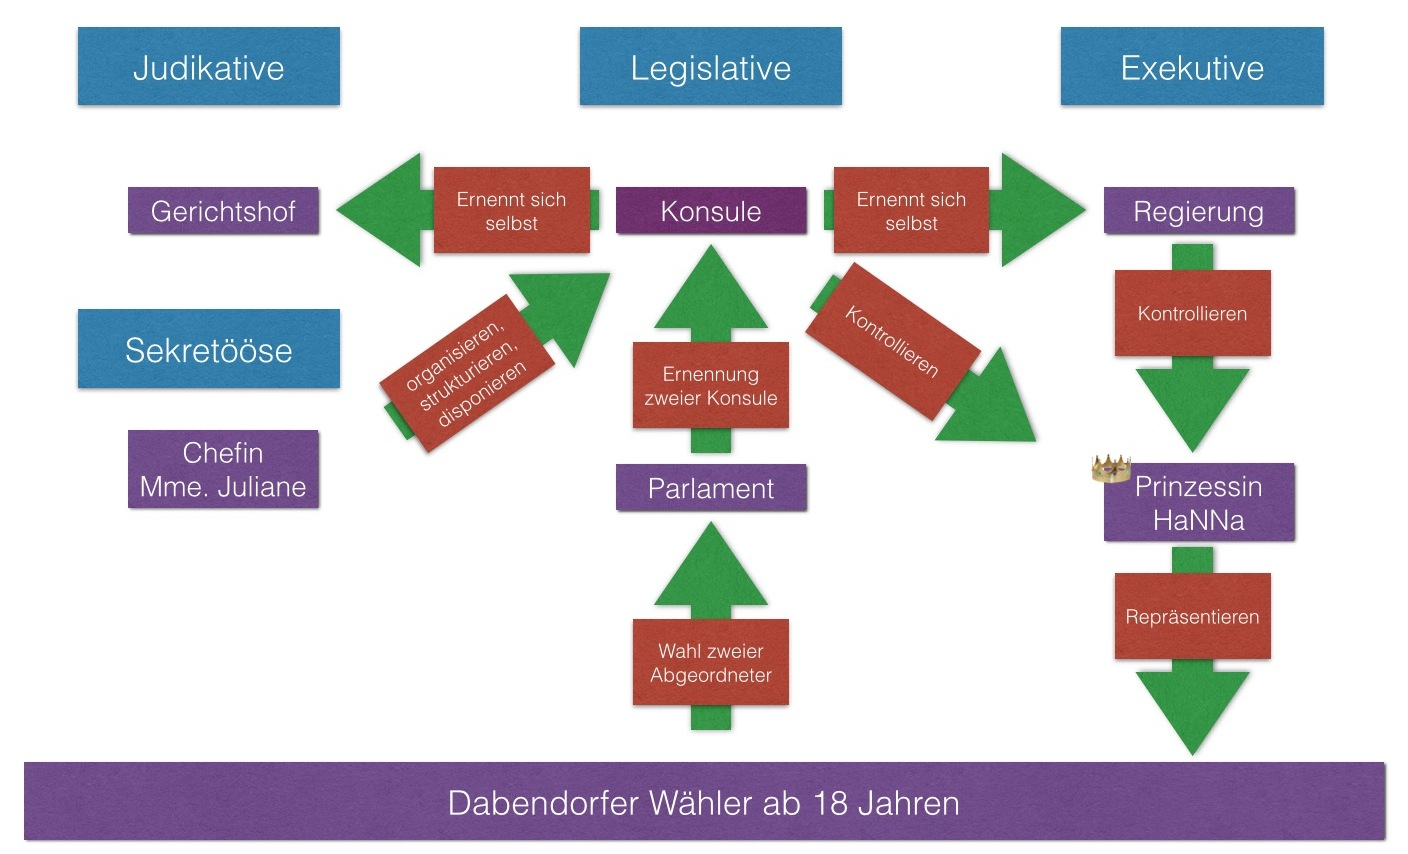
\includegraphics[width=0.95\textwidth]{bilder/gewaltenteilung.jpg}
\caption{Staatsaufbau Dabendorfs nach Gewalten}
\end{figure}
\noindent Der \textit{Dabendorfer Staat} besitzt einen hochkomplexen und in vielen Millionen Zeiteinheiten durch \textit{N} entwickelten Staatsaufbau, der durch seinen \textit{bürokratiearmen}, aber zugleich \textit{höchst effektiven Stil} im Gegensatz zu früheren Systemen und dem System im \textit{Franzakenreich} heraussticht. Eine \textit{Gewaltenteilung} nach den Theorien von Baron de Montesquieu wurde in seriöserer Art und Weise \textit{modifiziert} und umfasst nun neben der \textit{Legislative, einer Exekutive und der Judikative auch die Dabendorfer Sekretööse}, welche alle relevanten \textit{Aufgaben in Dabendorf verwaltet und ausführt}. Das System und seine Mitglieder werden alle \textit{42 Trillionen Jahre durch Wahlen bestätigt}, bei denen alle \textit{Dabendorfer Wähler ab 18 Jahren wahlberechtigt} sind. Wähler Dabendorfs sind alle \textit{mehrzelligen Lebensformen des Planeten Erde}, die \textit{keine Franzakische Staatsbürgerschaft} besitzen. Die Begrenzung des Wahlalters auf 18 Jahre ist ein Relikt früherer Zeiten, als es noch Kinder in Dabendorf gegeben hat. Das Wahlintervall von 42 Trillionen Jahren hat sich aus der Tatsache heraus ergeben, dass \textit{Dabendorfer unsterblich} sind (siehe \textit{\nameref{todsterben}}) und sich kleinere Intervalle als verwaltungstechnisch ineffektiv gezeigt haben. Die \textit{Wähler Dabendorfs wählen} zu den stattfindenden Wahlen insgesamt \textit{zwei Abgeordnete für das Parlament Dabendorfs}. Selbiges \textit{Parlament wählt aus den zwei Abgeordneten insgesamt zwei Abgeordnete} nach einer Kampfabstimmung aus ($\binom{2}{2}$), welche fortan die \textit{Konsule Dabendorfs} darstellen. Die \textit{Konsule Dabendorfs besitzen alle Gewalt der Gesetzgebung in Dabendorf}. Da sie jedoch per definitionem \textit{prokrastinativ arbeitsfern} sind, geben sie ihre Kompetenzen an andere Gewalten ab. Sie bilden die \textit{Dabendorfer Regierung} und kontrollieren die \textit{Prinzessin von Dabendorf}\footnote{Prinzessin von Dabendorf ist ein Eigenname und stammt aus der Zeit vor der Regelung der weiblichen Sprachformen des Dabendorferischen. Der korrekte Term würde in Neudabendorfer Sprache daher \enquote{Prinzööse von Dabendorf} heißen.}. Selbige ist durch \textit{N} höchstpersönlich ernannt worden und \textit{repräsentiert das Dabendorfer Volk}. Die \textit{Prinzessin von Dabendorf} bildet mit den \textit{beiden Konsulen} zusammen die \textit{Päpstliche Dabendorfer Kammer}. Die Konsule sitzen ferner auch im \textit{Dabendorfer Gerichtshof}, treffen alle ihre Entscheidungen jedoch im \textit{Konsensprinzip mit N}. Die eigentlichen \textit{Amtsgeschäfte Dabendorfs} führt jedoch die \textit{Sekretööse} aus, welche im Auftrag der Konsule \textit{organisiert, strukturiert und disponiert}. Sie wird durch die Dabendorfer Konsule nach einem \textit{Dabendorfweiten Casting} im Anschluss an die aktuellen Wahlen ernannt. Es wird jedoch hervorgehoben, dass die Mitglieder des Dabendorfer Verwaltungsapparates \textit{keinerlei Privilegien} zum restlichen Volk besitzen, keine obskuren Extragehälter beziehen und für die \textit{Umsetzung des Volkes Willen} verantwortlich sind.

\subsection{{Die drei Päpste}}
Die \textit{beiden Konsule und die Prinzessin von Dabendorf} bilden zusammen im Namen des \textit{N} die \textit{drei Dabendorfer Päpste}. Sie sind für die \textit{direkte Kommunikation des Volkes}, deren Vertreter sie sind, \textit{mit den großen Dabendorfer Göttern} verantwortlich. Sie besitzen einen direkten Draht zum großen \textit{N}, sind jedoch auch im Stande, innerhalb kürzester Zeit \textit{Kontakt zu Napoléon Bonaparte des Franzakenreichs} aufzunehmen. Sie fungieren als Vertreter des \textit{N} auf Erden, besitzen jedoch \textit{keinerlei außerordentlichen Fähigkeiten}, die \textit{N} besitzt. Ferner sind sie \textit{Verwalter des nationalen Süßkramvorrats} und dafür verantwortlich, dass jeder Bürger Zugriff darauf erhält, ohne dass feindliche Mächte selbigem Schaden zufügen können. Ihr Hauptsitz ist in der \textit{Dabendorf Orthodoxen Kathedrale in Dabendorf City}, in welche sie sich oft einige Zeitintervalle zur individuellen \textit{Prokrastination} zurückziehen.

\subsection{{Die zwei Konsule}}
Die \textit{Dabendorfer Konsule} sind direkt durch das vom Volk gewählte Parlament legitimiert und bilden die \textit{Regierung Dabendorfs}, deren Aufgaben sie an Handlanger und ihre große \textit{Sekretööse von Dabendorf} weitergeben. Sie sind dem \textit{Maltismus-Dabendorfismus} verschrieben und beauftragt, den \textit{Willen des Volkes} umzusetzen. Sie sind die \textit{Gesichter einer antikapitalistischen Regierung}, frei vom Einfluss anderer obskurer Religionen. Nach ihrem \textit{Sieg bei den Wahlen Dabendorfs} sind sie per Gesetz verpflichtet, dem gesamten Wahlvolk einen \textit{Vorrat von Kaffee, Hallorenkugeln und anderem Süßkram} zu verschaffen, der bis zur nächsten Wahl ausreichend vorliegt. Additional dazu ist es ihre \textit{Verantwortung, an jedem Dabendorfer Feiertag} durch den \textit{offiziellen Dabendorf Orthodoxen Gottesdienst} zu führen und den \textit{Segen des N} auf alle Individuen zu verteilen. Eine ihrer wichtigsten Aufgaben ist es auch, \textit{diplomatische Beziehungen zum Franzakenreich} aufzubauen und zu pflegen, sowie den \textit{Staatshaushalt Dabendorfs im Sinne des Maltismus-Dabendorfismus zu verwalten} und \textit{von Kapitalismus und Korruption fernzuhalten}.\\
Amtierende \textit{Konsule von Dabendorf} sind \textit{Malte und Lukas von und zu Dabendorf City}, unterstützt durch ihre \textit{zauberhaften Gattöösen Franzi und Nathi}.

\subsubsection{{Gattööse Nathi}}
Die \textit{ultimativ süß-knuffige Nathi} ist die \textit{liebevoll putzige Gattööse des Papstes Lukas von Dabendorf City}, die seit mehreren Millionen Dabendorfer Zeiteinheiten liebevoll an seiner Seite agiert. Ihr \textit{Verhältnis zu Einhörern ist positiv bis knorke} und ihre \textit{Knuffigkeit grenzenlos}. Sie besitzt das \textit{Dabendorfer Diplom der Meisterstochastikerin} und ist die erste Person der DOR, bei welcher eine \textit{Redegeschwindigkeit} mit reichhaltigem Inhalt gemessen wurde, die \textit{schneller als ein durchschnittlicher Wasserfall} bei $9,81 \frac{m}{s^2}$ Fallbeschleunigung ist. Ferner ist sie \textit{Halterin zahlreicher Dabendorfer Sportrekorde} und konträr zu ihrem Gatten und der Dabendorfer Allgemeinheit durch spezifisch obskure Gene zu \textit{athletischen Höchstleistungen fähig}. Die Limes der \textit{ehelichen Liebe tendiert gegen unendlich} und ermöglicht die einmalige Produktion einer gigantischen Menge an \textit{Bussys}, mit denen das Dabendorfer Volk versorgt und \textit{grenzenlos glücklich} gehalten wird. Ihr spezifisch skandalöser \textit{Hang zum Konsum obskurer Serieninhalte} des \textit{bösen Unkle Sams} sind es jedoch, die ihren Gatten in große Angst versetzen und bestürzend \textit{gruselige Essenz in die Ehe fusionieren}.

\subsubsection{{Gemahlin Franzi}}
\textit{Genossin Franzi} ist die fabulöse \textit{Angetraute des Papsts und Konsuls Malte}, welche in einer streng geheimen Nacht-und-Nebel-Aktion in den \textit{abtrünnigen Gebieten Schottlands} unter mysteriösen Umständen in eine \textit{Ehe} mit selbigem integriert wurde. Sie vertritt \textit{antagonistische Eigenschaften zum Dabendorfer Papst Malte} und ist daher stets für Momente zuständig, die die Dabendorfer Konsule in ihren Grundfesten erschüttern. So vertritt sie \textit{Kreativität, Pünktlichkeit und Opportunismus} in gleich schockierendem Maße und ist auf ähnlich \textit{antiprokrastinativen Wegen} wie die Sekretööse Jane unterwegs. Ferner ist sie \textit{kaffeeabhängig} und vertritt die \textit{künstlerisch-kreativ-musikalische Ebene Dabendorfs}, zumindest diejenige, die nicht schon durch die \textit{phänomenale Raffinesse von Malte und Lukas} abgedeckt ist. Überdies ist additional zu erwähnen, dass sie die magische Gabe besitzt, über einen längeren Zeitraum neben \textit{Dabendorfer Geistlichen} zu sitzen und \textit{Integrale sowie Binomialverteilungen} zu knacken, ohne skandalös zu scheitern.

\subsection{{Prinzessin HaNNa}}
Die \textit{Dabendorfer Prinzessin besitzt repräsentative Zwecke} im Staate und erscheint auf allen relevanten \textit{staatlichen Feiertagen} zur \textit{Zelebration mit dem Dabendorfer Volk}. Sie ist durch \textit{N} höchstpersönlich ernannt und bewegt sich \textit{reitend auf dem Dabendorfer Einhorn Kathi} fort, um ihren zerstörten Rücken instand zu halten. In ihren \textit{Haaren} bewahrt sie allerlei relevanten Krimskrams auf, da sie ein Verfassungsvermögen von über \textit{42 Kubikeiffelturmhöhen} haben. Sie besitzt als einzige Person das \textit{staatlich anerkannte Apfelkuchendiplom} und vertreibt ihre \textit{Apfelkuchen zum Nulltarif} in der großen Kantine des \textit{Dabendorfer Schlosses}, in welchem sie auch residiert. Zu jedem essentiellen Ereignis tritt sie morgens auf dessen Balkon und \textit{wirft Süßkram in die jubelnde Menge}. Sämtliche ihrer \textit{Klamotten} werden durch den \textit{Dabendorfer Stardesigner Malte höchstpersönlich aus roter und DORgrüner Wolle handgehäkelt} und spezialangefertigt. Sie ist die \textit{meist gegooglete Person des Dabendorfer Staates und besitzt Kultstatus in Dabendorfer Souvenirläden}. Amtierende Prinzessin von Dabendorf ist \textit{Ihre Königliche Majestät Prinzessin Mademoiselle HaNNa Elfriede CoriNNa Tebartz von und zu Dabendorf City}. Die Tatsache, dass sie bisher über \textit{keinen Prinzen} verfügt ist der Grund, warum landesweit nach dem bestpassenden männlichen Pendant gesucht wird. Qualifiziert auf selbiges Amt sind nach Definition des \textit{N} jedoch nur diejenigen, die neben den \textit{Konsulen Malte und Lukas} nach dem \textit{Dabendorfer Beziehungsalgorithmus} zu mindestens 99\% der \textit{Prinzessin} zugehörig sind. Ferner muss er im Stande sein, die \textit{Dabendorfer Konsule} und \textit{N} in \textit{mindestens zwei der drei Disziplinen Schach, Bankbowling und Bridge zu besiegen}. Die \textit{Legende} besagt, dass dieser Mensch nur \textit{einmal auf der Erde existiert}, von seinem Glück aber selbst noch nichts weiß. Die Suche des \textit{Prinzen von Dabendorf} beschäftigt mehrere \textit{hundert Wissenschaftler in ganz Dabendorf}.

\clearpage

\subsection{{Einhorn Kathi}}
Das \textit{Dabendorfer Einhorn Kathi} ist das \textit{zauberhafteste Wesen Dabendorfs}, neben den \textit{großen drei Göttern der DOR}. Es ist \textit{persönlicher Begleiter der Prinzessin HaNNa} und für ihre \textit{Sicherheit und den Transport ihrer Person} zuständig. Das Einhorn trägt \textit{pinkes, gut gepflegtes Fell, einen langen DORgrünen Schweif und das große Horn auf dem Kopfe}. Außerdem besitzt es im \textit{Bauch} einen großartigen, \textit{magischen Ofen}, welcher im Stande ist, auf Knopfdruck in kürzester Zeit \textit{Unmengen an Apfelkuchen und Pizza zu produzieren}. Über selbigen Kreislauf ist das Einhorn auch fähig, sich selbst \textit{ohne Energieaufnahme mit Nahrung zu versorgen}. Es ist daher das einzige Wesen auf der Welt, welches dem \textit{Energieerhaltungssatz vehement widerspricht}. Die \textit{Herkunft der Kathi} ist durch eine \textit{geheimnisvolle Legende der Dabendorfer Mythologie überliefert}, welche eines der größten \textit{Rätsel des Dabendorfismus} darstellt. Auf einem großen \textit{DORgrünen Feld hinter der Hauptstadt Dabendorf City} befindet sich ein \textit{großer Kreis mit 42 versteinerten Einhörnern} und einer \textit{kleinen Tafel in der Mitte}. Im Volksmund wird dieser Komplex auch \textit{DabenHenge} genannt. Diese 42 Einhörner sollen der Überlieferung nach die \textit{Ureinwohner Dabendorfs} gewesen sein, welche glücklich und gigaknorkulös gelebt haben. Ihr Leben soll jedoch durch ein \textit{schreckliches Großereignis} abrupt beendet worden sein, weshalb sie seitdem \textit{versteinert in diesem Kreis} stehen würden. Anlass und Ursachen dieses Großereignisses sind nicht bekannt, da die Einhörner die einzigen Lebewesen gewesen sind, die zu diesem Zeitpunkt \textit{N} existiert haben. \textit{N} selbst kann sich daran \textit{nicht mehr erinnern}. Die in der Mitte des Kreises befindliche \textit{Steintafel} gibt wenig Aufschluss auf selbigen Hergang. Auf ihr abgebildet sind ein \textit{Geldschein, eine Franzakische Flagge und ein Text in einer völlig unbekannten, geheimnisvollen Sprache}, der mit \enquote{Il était une fois...} beginnt. Der Legende nach hat lediglich ein \textit{kleines Ei das große Unglück überlebt}, aus welchem später das \textit{Babyeinhorn Kathi} schlüpfte. Es war selbst zu jung, um sich daran heute erinnern zu können. \textit{Einhorn Kathi} ist dieser Theorie folgend auch das \textit{älteste Wesen in ganz Dabendorf}, obwohl es keine Alterserscheinungen zeigt.\\
Einem \textit{Dabendorfer Märchen} zufolge besitzt die \textit{Steintafel im Kreis eine kleine Vertiefung}, deren Betätigung einen \textit{Chemiebaukasten} zum Vorschein bringt. Nach korrekter \textit{Zusammenmischung verschiedener Substanzen} würde \textit{Licht aus einem der Reagenzgläser} schießen. \textit{Napoléon Bonaparte} behauptet, sich beim bisher einzigen Vorkommnis dieser Art \textit{in das Licht gestellt} zu haben und seitdem seine \textit{ultimativen Kräfte zu besitzen}. Im \textit{Heimatmuseum in Paris} befinden sich \textit{angebliche Beweise} hierfür, nämlich eine \textit{Menge an Fleischbällchen und Gesteinsbrocken}, die damals vom Himmel geregnet haben sollen.

\subsection{{Sekretööse Jane}}
Die \textit{magische Sekretööse Jane} ist für den Verwaltungsaufbau Dabendorfs von \textit{ultimativ relevanter Bedeutung}. Sämtliche Verwaltungstätigkeiten, für die die \textit{Dabendorfer Päpste Malte, HaNNa und Luki} viel zu bequem sind werden von ihr ausgeführt. Aufgrund der \textit{Prokrastinationskrankheit}, an welcher die DORs leiden, sind dies eine ganze Menge Inhalte. Die Sekretööse Jane ist die \textit{einzige bekannte Dabendorferin mit dem Diplom im Antiprokrastinations- und Verwaltungswesen}. Ihr Genmaterial ist so aufgebaut, dass sie der \textit{Prokrastination widerstehen} kann und unermüdlich weiter arbeitet. Damit ist sie das \textit{essentiellste Glied} des kleingehaltenen Bürokratieakts Dabendorfs. Ferner reagiert sie allergisch gegen Freizeit und \textit{arbeitet vierundzwanzig Stunden am Tag für den Erhalt Dabendorfs}. Ihre Energie generiert sie aus dem \textit{Stromkabel}, welches ihr aus dem Rücken heraus ragt und stets an den nächstgelegenen \textit{Apfelkuchenofen} angeschlossen werden muss. Ein entsprechender \textit{Transformator} hierfür ist in allen Dabendorfer Baumärkten erhältlich. Als Abfallprodukt ihrer guten Arbeit und des Hass auf Prokrastination entsteht ein \textit{Gemisch aus Groll über die prokrastinative Masse}, weshalb sie ein \textit{einzigartiges Unterhaltungsprogramm durch die DORkonsule} genießt, um an Effektivität und Raffinesse nicht zugrunde zu gehen. Trotz ihrer vielen Aufgaben ist die Sekretööse jedoch bei weitem \textit{nicht ausgelastet}. Um wirklich 24 Stunden am Tag arbeiten zu können, vertieft sie sich in das \textit{Studium all jener Denker, deren Erkenntnisse bald obsolet werden}. Vor allem der für seine \textit{wissenschaftliche Irrelevanz} bekannte {\tiny Sigmund Freud} genießt enorme zeitliche Zuwendung. Diese Art von Beschäftigung bezeichnen Wissenschaftler auch als ihre \textit{eigentliche Prokrastination}, welche durchaus Schnittmengen mit der ihr genetisch verwehrten prokrastinativen Materie aufweist. Additional sind ihre \textit{manipulativen Fähigkeiten} zu erwähnen, welche es ihr ermöglichen, sich auch durch \textit{sexistische Aspekte und umkehrpsychologische Gegebenheiten einen Vorteil gegenüber anderen Dabendorfern zu beschaffen}, der auf Außenstehende obskur ungerecht wirken kann. Ferner ist eines der weltberühmten \textit{Weltuntergangsszenarien} ist als \textit{Big Jane} bekannt. Dieses umfasst die Theorie, dass \textit{Jane mehrere Tage in Folge prokrastiniert} und nicht die Aufgaben wahrnimmt, die man ihr aufträgt. Rein logisch ist diese \textit{Szene nicht erklärbar}, daher datieren Forscher diesen Tag als \textit{möglichen Zeitpunkt eines Weltuntergangs}, welcher zuerst alle Prokrastinaten mit in die Tiefe reißen würde.

\subsection{{Flagge und Wappen Dabendorfs}}
\vspace*{-3mm}
\begin{figure}[!ht]
\centering
\begin{floatrow}
\ffigbox[\FBwidth]{\caption{Dabendorfer Flagge}}{

\includegraphics[width=0.5\textwidth]{bilder/dorflagge.png}
}
\ffigbox[\FBwidth]{\caption{Dabendorfer Wappen}}{

\includegraphics[width=0.5\textwidth]{bilder/doreinhorn.jpg}
}
\end{floatrow}
\end{figure}
\vspace*{-2mm}
\noindent Die beiden \textit{Dabendorfer Nationalsymbole}, die \textit{Flagge und das Wappen}, besitzen in ihrer offiziellen Größe die \textit{Proportionen von 3,14 zu 2,71} ($\pi : e$). Die \textit{Dabendorfer Flagge} stellt ein \textit{DORgrünes N auf DORgrünem Grund} dar. Der \textit{DORgrüne Grundton} ist definiert als \textit{\#33B200}. Die \textit{Magie in der Flagge} besteht darin, dass jeder Dabendorfer Bürger das \textit{N} an einer völlig anderen Stelle sieht, als seine vielen Mitbürger. Außerdem ist sie selbst durch kreativ ungünstig veranlagte Menschen \textit{mit leichten Mitteln zu reproduzieren und gut zu merken}. Ein jedes \textit{Dabendorfer Verwaltungsgebäude} hat mindestens eine Dabendorfer Flagge über seinem Eingang zu wehen. Das \textit{Wappen} hingegen stellt das \textit{Symbol der Prinzessin HaNNa} und des \textit{Einhorn Kathis} dar. Abgebildet ist eine \textit{weiße Silhouette des Dabendorfer Einhorns} auf einem Hintergrund, der dunkler als das angestammte DORgrün ist. Außerdem ist im weißen Einhorn in selbigem Farbton ein \textit{großes geschwungenes N} abgebildet. Das \textit{Dabendorfer Wappen} ziert neben dem \textit{Königshaus} auch alle \textit{offiziellen Dabendorfer Dokumente und durch N herausgegebenen Glaubensschriften}.

\section{{Maltismus-Dabendorfismus}}
Zum Zeitpunkt 6.062.013.945 \footnote{greg. 10.06.2013; siehe \nameref{DabendorferKalender}} erschien das renommierte Magazin \textit{N und die Welt}. Ein \textit{Kompendium der faszinierendsten und relevantesten Informationen aus Dabendorf} und sogar dem Franzakenreich. In einer nun sehr berühmten Ausgabe jedoch erschien neben Berichten über das Zeitgeschehen auch ein Artikel der aus der Perspektive des Zeitpunktes 9.372.409.200 \footnote{greg. Jahr 2118} die \textit{globale wirtschaftliche Entwicklung der Zeitspanne [6.216.735.600, 9.372.409.200] \footnote{greg. 2018 bis 2118}} analysierte. Die dort beschriebenen Katastrophen und Großartigkeiten erregten viele Wissenschaftler zum Wundern und die gesamte Medienlandschaft zu einer intensiven Berichtserstattung. Lange wusste keiner, wo dieser Artikel seinen Ursprung hatte. War es eine von \textit{Napoléon gesäte Falschinformation}? Handelte es sich um eine \textit{Prophezeiung, die einem Reporter von N eingeflößt} wurde? Oder war es ein Weg, die letzten fehlenden Seiten des Magazins zu füllen, ohne lange die \textit{Prokrastination} der Schreiber zu unterbrechen?\\
Lange \textit{Analysen durch die päpstlichen Theoretiker} brachten die Antwort. Es handelte sich allem Zweifel zum Trotz um eine womöglich \textit{wahrheitsgetreue Vision des DOR-Konsuls Malte}. Dieser hatte versehentlich \textit{Bierdeckel mit seinem Kaffee zu sich genommen} und war in einen \textit{Rausch der Einsicht} abgerutscht, ohne dies zu realisieren. In Konsequenz zu diesen Ereignissen und Erkenntnissen gab es einen \textit{globalen Aufruhr}. Man munkelte über die möglichen Kollateralschäden der völlig freien Marktwirtschaft sowie die elende Katastrophe der \enquote{Black Decision}, jedoch gab es auch eine immense Hoffnung auf die verfrühte Einführung des \textit{Malleus Economicarums} ({dab. \enquote{Der Wirtschaftshammer}}). Sich all dieser Bedenken und Wünsche annehmend traf sich die \textit{interne Spitze der DOR} und lies unter strenger Aufsicht ein \enquote{Malleus Economicarum} ausarbeiten, welches keine vorhergehende Unterdrückung braucht und trotzdem all das bietet, was die Prophezeiung versprach. Der \textit{Maltismus-Dabendorfismus} ward geboren.\\[0.5cm]
%[Einfügung des Original Malleus Eco.]
Die \textit{Grundsätze} dieses ultimativ knorken Wirtschaftssystems lassen sich in \textit{wenigen Unterpunkten} zusammenfassen:
\begin{itemize}
\item Der \textit{Maltismus-Dabendorfismus} orientiert sich an vielen \textit{kommunistischen} und vereinzelten sozialistischen Strömungen der vergangenen fünf Milliarden Zeiteinheiten. Einzelne \textit{Fehler} können jedoch durch Anwendung gezielter Systeme \textit{überwunden} werden.
\item \textit{Recht auf Arbeit}:\\
Arbeiten macht viele Menschen glücklich, andere können nur zufrieden sein, solange sie \textit{effektiv prokrastinieren} können. Deswegen setzen sich die \textit{Päpstlichen Eminenzen} schon lange für ein \textit{Recht auf Arbeit} ein. Selbige floss auch direkt in diese neue \textit{Wirtschaftsordnung} ein. In Bereichen wie \textit{Messdienst, Wissenschaft und Programmieren} steht jedem Dabendorfer immer die Tür offen.
\item \textit{Forschung}:\\
Das \textit{Dabendorfer System} ist das erste System, in welchem \textit{Kapazitäten existent} sind, sich mit \textit{seriöser Wissenschaft} zu befassen, die nicht ausschließlich zur Entwicklung neuer Kriegswaffen angewandt wird, wie es im \textit{US-amerikanischen Kapitalismus} üblich war. Die \textit{Steckeneinhörner Intellektueller} sind die \textit{Forschung an besserem Essen, einem seriösen Java-Compiler sowie der \nameref{FranzGenom}}.
\item \textit{Arbeitspflicht}:\\
Viele sozialistische Regime mussten zum Überleben ihre Bürger zum Arbeiten zwingen. Ein \textit{ausgefuchstes System von höchst wissenschaftlicher Methodik und dramatischer Einhorn-Magie} ermöglichen es den Dabendorfern jedoch alle \textit{körperlichen Notwendigkeiten abzudecken}, \textit{ohne} dass es nur den \textit{geringsten menschlichen Aufwand} bedarf. Als Konsequenz können wir den \textit{ultimativ faulsten Lebewesen} garantieren, dass \textit{Arbeiten nie notwendig} ist.\\
Man könnte hierbei von einem \textit{bedingungslosen Grundeinkommen} sprechen. Dieser Begriff wäre jedoch zu weit hergeholt, wenn man bedenkt, dass der \textit{Begriff Einkommen als solches in einer gigaknorken kapitalfreien Gesellschaft nicht mehr erforderlich} ist.
\item \textit{Bezahlung}:\\
Die meisten \textit{Kommunismustheorien} befassen sich hauptsächlich mit den \textit{Problematiken von Geld}. Dies ist \textit{im Maltismus-Dabendorfismus nicht notwendig}. Eine \textit{immense Produktionsgeschwindgkeit} erlaubt es zu jeder Zeit alle \textit{Güter zur Bedürfnisbefriedigung} bereit zu stellen. Engpässe, also den \textit{Bedarf zum Handeln kann es deswegen also nie geben}. \textit{Geld verliert alle Bedeutung}. Im Kapitalismus Wirklichkeit gewordene skandalöse Tatsachen wie die Erzählungen von \textit{George Orwell} und die stetige \textit{Knappheit} können \textit{im modernen Maltismus-Dabendorfismus ad acta gelegt} werden.\footnote{Die gigantische Produktionsgeschwindigkeit, die sich selbst \textit{knechtende Bourgeoise} nie vorgestellt hätten kommen nicht durch menschenunwürdige Ausbeutung, sondern durch \textit{cleverste Utilisierung der Dabendorfer Einhornpower und Schaffung neuer Java-Problemlösungsansätze}.}
\end{itemize}
In allen weiteren ideologischen Merkmalen unterscheidet der \textit{Maltistisch-Dabendorfistische Ansatz} sich nicht sehr vom marxistisch geprägten Kommunismus. Bei Fragen zu \textit{Risiken und Nebenwirkungen} lesen Sie bitte den bald erscheinenden \textit{Almanach der Wirtschaftsfrage} oder fragen Sie Ihren \textit{Papst oder Konsul}.\footnote{Der Almanach der Wirtschaftsfrage ist das bald erscheinende \textit{Hauptwerk des N}, worin dieser seine \mbox{Ultimativtheorie} des endgültigen \textit{Maltismus-Dabendorfismus} formuliert und ferner Stellung zu \textit{\mbox{Pikettys} Werken} bezieht.}

\subsection{{Kapitalakkumulationskritik}}
\textit{Dabendorf} steht in einer langen Reihe von \textit{Kapitalismuskritikern und Kommunisten}, die mit bedauerndem Auge und scharfem Wort die \textit{Kapitalakkumulation der Kapitalisten} betrachten. \textit{N und seine Jünger} sind sich im Klaren über die \textit{große Gefahr}, die für alle im Schatten der \textit{Bestie des Geldes} lebenden Menschen und Franzaken gilt. In den Zeiten bis zur \textit{Revolution des Dabendorfer Systems} galt es deswegen auch als schreckliche Sünde, sich mit diesem scheußlichen Laster zu beschäftigen und ein \textit{Beweis der Quadratur des Kreises} wurde unmittelbar nötig. Die Einführung des \textit{Maltismus-Dabendorfismus} jedoch macht es zu einer \textit{Unmöglichkeit in Dabendorf lokal Kapital zu akkumulieren}.\\
Der wahre Kapitalist, findig in seiner Methodik, erkennt jedoch schnell, dass das \textit{Franzakenreich} keinesfalls dieselbe \textit{wunderbare Malt.-Dabend. Ordnung teilt, durch die Dabendorf floriert} und wächst. Im Land jenseits des Elsass besteht immer noch die Möglichkeit zu kaufen und zu verkaufen. Der \textit{Kapitalakkumulation ist somit ein letztes Tor offen}.\\
Doch gebet Acht, \textit{Monster des Kapitalismus}! In \textit{Dabendorf und all seinen Provinzen ist es strengstens verboten, Kapital zu akkumulieren}. Die diplomatischen Beziehungen zu den Franzaken gebieten es jedwede Einschränkung ihrer Funktionstüchtigkeit zu dulden oder zu ermuntern. Es sei des Weiteren gesagt, dass \textit{Napoléon} selbst eine \textit{Einschränkung in der Funktionsfähigkeit seines geliebten Vaterlandes nie dulden würde} und auf den Verbrecher \textit{schlimmeres als die Quadratur des Kreises} warten würde.